\documentclass[11pt, dvipsnames, handout]{beamer}
\newtoggle{full}
\settoggle{full}{true}

\newtoggle{covered}
\settoggle{covered}{false}

\newtoggle{presentable}
\settoggle{presentable}{false}

\newtoggle{dualscreen}
\settoggle{dualscreen}{false}

\usepackage{pgfplots}
%\pgfplotsset{compat = newest}

\usepackage{pgfpages}

\setbeamertemplate{note page}{\pagecolor{yellow!5}\vfill \insertnote \vfill}
\usepackage{collect}
\definecollection{notes}
\newcounter{notestaken}

\usepackage{xpatch}

\usepackage{ulem}

\usepackage[framemethod=tikz]{mdframed}

\usepackage{scalerel}
\usepackage{calc}

%\usepackage{enumitem}
\setlength\fboxsep{.2em}

\usepackage{graphicx} % Allows including images
\usepackage{booktabs} % Allows the use of \toprule, \midrule and \bottomrule in tables

\xpatchcmd{\itemize}
  {\def\makelabel}
  {\setlength{\itemsep}{0.65 em}\def\makelabel}
  {}
  {}


\xpatchcmd{\beamer@enum@}
  {\def\makelabel}
  {\setlength{\itemsep}{0.65 em}\def\makelabel}
  {}
  {}


%\makeatletter
%\renewcommand{\itemize}[1][]{%
%  \beamer@ifempty{#1}{}{\def\beamer@defaultospec{#1}}%
%  \ifnum \@itemdepth >2\relax\@toodeep\else
%    \advance\@itemdepth\@ne
%    \beamer@computepref\@itemdepth% sets \beameritemnestingprefix
%    \usebeamerfont{itemize/enumerate \beameritemnestingprefix body}%
%    \usebeamercolor[fg]{itemize/enumerate \beameritemnestingprefix body}%
%    \usebeamertemplate{itemize/enumerate \beameritemnestingprefix body begin}%
%    \list
%      {\usebeamertemplate{itemize \beameritemnestingprefix item}}
%      {%
%        \setlength\topsep{1em}%NEW
%        \setlength\partopsep{1em}%NEW
%        \setlength\itemsep{1em}%NEW
%        \def\makelabel##1{%
%          {%
%            \hss\llap{{%
%                \usebeamerfont*{itemize \beameritemnestingprefix item}%
%                \usebeamercolor[fg]{itemize \beameritemnestingprefix item}##1}}%
%          }%
%        }%
%      }
%  \fi%
%  \beamer@cramped%
%  \raggedright%
%  \beamer@firstlineitemizeunskip%
%}
%
%
%
%
%
%\makeatother

%\setlist[beamer@enum@]{topsep=1 em}
%\let\origcheckmark\checkmark %screw you dingbat
%\let\checkmark\undefined %screw you dingbat
%\usepackage{dingbat} 
%\let\checkmark\origcheckmark %screw you dingbat






%\usepackage{fontawesome}

\usepackage{mathtools}
\usepackage{etoolbox, calculator}

\usepackage{xcolor}
\usepackage{tikz}
\usetikzlibrary{arrows.meta}
\usetikzlibrary{calc}
\usepackage[nomessages]{fp}
\usepackage{transparent}
\usepackage{accsupp}
%\usepackage{color, xcolor}

%colorblind-friendly palette
%\definecolor{dblue}{RGB}{51,34,136}
\definecolor{lblue}{RGB}{136,204,238}
%\definecolor{green}{RGB}{17,119,51}
\definecolor{tan}{RGB}{221,204,119}
%\definecolor{mauve}{RGB}{204,102,119}

\usepackage{tcolorbox}



\usepackage{xifthen}
\usepackage{nicefrac}
\usepackage{amsmath}
\usepackage{amsthm}
\usepackage{amssymb}
\theoremstyle{definition}
\newtheorem*{define}{Definition}
\newtheorem*{recall}{Recall}


\DeclareMathOperator{\tr}{tr}

\usepackage{multicol}
%\setlength{\columnsep}{1cm}

\usepackage{tablists, amsmath,vwcol, cancel, polynom}
\usetikzlibrary{shapes, patterns, decorations.shapes}
%\usepackage{tikzpeople}
\tikzstyle{vertex}=[shape=circle, minimum size=2mm, inner sep=0, fill]
\tikzstyle{opendot}=[shape=circle, minimum size=2mm, inner sep=0, fill=white, draw]

% common math quick commands
\newcommand{\nicedd}[2]{\nicefrac{\text{d}#1}{\text{d}#2}}
\newcommand{\dd}[2]{\dfrac{\text{d}#1}{\text{d}#2}}
\newcommand{\pd}[2]{\dfrac{\partial #1}{\partial#2}}
\renewcommand{\d}[1]{\text{d}#1}
\newcommand{\ddn}[3]{\dfrac{\text{d}^{#3}#1}{\text{d}#2^{#3}}}
\newcommand{\pdn}[3]{\dfrac{\partial^{#3}#1}{\partial#2^{#3}}}
\newcommand{\p}[0]{^{\prime}}
\newcommand{\pp}[0]{^{\prime\prime}}
\newcommand{\op}[2][\text{L}]{#1 \left[ #2 \right]}

\newcommand{\lap}[1]{\mathcal{L}\left\{#1\right\}}
\newcommand{\lapinv}[1]{\mathcal{L}^{-1}\left\{#1\right\}}
\newcommand{\lapint}[1]{\int_0^\infty e^{-st}#1dt}
\newcommand{\evalat}[2]{\Big|_{#1}^{#2}}

\newcommand{\paren}[1]{ \left( #1 \right)}

\newcommand{\haxis}[4][\normcolor]{\draw[#1, <->] (-#2,0)--(#3,0) node[right]{$#4$}; }


\newcommand{\axis}[4]{\draw[\normcolor, <->] (-#1,0)--(#2,0) 
node[right]{$x$};
\draw[help lines, <->] (0,-#3)--(0,#4) node[above]{$y$};}

\newcommand{\laxis}[6]{\draw[<->] (-#1,0)--(#2,0) 
node[right]{$#5$};
\draw[ <->] (0,-#3)--(0,#4) node[above]{$#6$};}
\newcommand{\xcoord}[2]{
	\draw (#1,.2)--(#1,-.2) node[below]{$#2$};}
\newcommand{\textnode}[3]{
	\draw (#1,#2) node[below]{$#3$};}
	
\newcommand{\nxcoord}[2]{
	\draw (#1,-.2)--(#1,.2) node[above]{$#2$};}
\newcommand{\ycoord}[2]{
	\draw (.2,#1)--(-.2,#1) node[left]{$#2$};}
\newcommand{\nycoord}[2]{
	\draw (-.2,#1)--(.2,#1) node[right]{$#2$};}
\newcommand{\dlim}{\displaystyle\lim}
\newcommand{\dlimx}[1]{\displaystyle\lim_{x \rightarrow #1}}
\newcommand{\stickfig}[2]{
	\draw (#1,#2) arc(-90:270:2mm);
	\draw (#1,#2)--(#1,#2-.5) (#1-.25,#2-.75)--(#1,#2-.5)--(#1+.25,#2-.75) (#1-.2,#2-.2)--(#1+.2,#2-.2);}	

%\newcounter{example}
%\setcounter{example}{1}
%\newcounter{preFrameExample}
%\AtBeginEnvironment{frame}{\setcounter{preFrameExample}{\value{example}}}
%\newcommand{\ex}[1]{
%	 \setcounter{example}{\value{preFrameExample}}
%	 \textcolor{green}{\small\fbox{Example \arabic{example}: #1}}\\[8pt]
%	\stepcounter{example}}
%\newcommand{\exans}[1]{
%	\SUBTRACT{\value{preFrameExample}}{1}{\n}
%	 \textcolor{green}{\small\fbox{Solution \n: #1}}\\[8pt]}
\mode<presentation> {

% The Beamer class comes with a number of default slide themes
% which change the colors and layouts of slides. Below this is a list
% of all the themes, uncomment each in turn to see what they look like.


\usetheme{CambridgeUS}
\usecolortheme[named=black]{structure}


\newcommand{\studentcolor}[0]{ForestGreen}
\newcommand{\normcolor}[0]{NavyBlue}
\newcommand{\alertcolor}{Red}

\setbeamercolor{normal text}{fg=\normcolor}
\setbeamercolor{frametitle}{fg=\normcolor}
\setbeamercolor{section in head/foot}{fg=Black, bg=Gray!20}
\setbeamercolor{subsection in head/foot}{fg=Green!70!Black, bg=Gray!10}
\setbeamercolor{alerted text}{fg=\alertcolor}
\setbeamerfont{alerted text}{series=\bf}
\setbeamertemplate{enumerate items}[default]
\setbeamercolor{enumerate item}{fg=\normcolor}

\setbeamertemplate{footline} % To remove the footer line in all slides uncomment this line
%\setbeamertemplate{footline}[page number] % To replace the footer line in all slides with a simple slide count uncomment this line

\setbeamertemplate{navigation symbols}{} % To remove the navigation symbols from the bottom of all slides uncomment this line
}

\newcommand{\alertbox}[1]{\tcbox[on line, colframe=\alertcolor, colback=White, left=2pt,right=2pt,top=2pt,bottom=2pt]{\usebeamercolor*{normal text}#1}}


\newcommand{\startstu}{\setbeamercolor{normal text}{fg=\studentcolor}\usebeamercolor*{normal text}\setbeamercolor{enumerate item}{fg=\studentcolor}\usebeamercolor*{enumerate item}}
\newcommand{\stopstu}{\setbeamercolor{normal text}{fg=\normcolor}\usebeamercolor*{normal text}\setbeamercolor{enumerate item}{fg=\normcolor}\usebeamercolor*{enumerate item}}

\newcommand{\takenote}[1]{ \begin{collect}{notes}{}{}{}{}  #1  \end{collect}  \addtocounter{notestaken}{1}} %\ifthenelse{\value{notestaken}>0}{\hrulefill\\}{}

\makeatletter
\newcommand{\cover}{\alt{\beamer@makecovered}{\beamer@fakeinvisible}}
\newcommand{\ucover}[1]{\iftoggle{full}{}{\beamer@endcovered}\stopstu#1\startstu\iftoggle{full}{}{\beamer@startcovered}}
\makeatother

\newcommand{\skippause}{ \addtocounter{beamerpauses}{-1}}
\newcommand{\blockpres}{ \skippause \pause }

\newcommand{\studentify}[1]{\startstu #1  \stopstu }
\newcommand{\student}[1]{\iftoggle{full}{ \pause  \studentify{#1} }{\iftoggle{covered}{\studentify{#1}}{\cover{  #1 }}}}
\newcommand{\cstudent}[1]{\student{\begin{center} #1 \end{center}}}
\newcommand{\fullonly}[1]{\iftoggle{full}{ #1}{}}
\newcommand{\presentonly}[1]{\iftoggle{presentable}{ #1}{}}

\usepackage{xparse}
\usepackage{xifthen}

% shortcuts for commonly-used presentation elements
%\NewDocumentCommand{\slide}{o m}
% {\IfValueTF{#1}{\begin{frame}[t]{#1}}{\begin{frame}[t]} #2 \end{frame}}

\newtoggle{iscovered}

\newcommand{\slide}[2][]{%
%\setcounter{notestaken}{0}
\takenote{#2} 
%\ifthenelse{\equal{#1}{}}{\begin{frame}[t]}{\begin{frame}[t]{#1}} #2 \ifthenelse{\value{notestaken}>0}{ \note{\includecollection{notes}}}{} \end{frame}%
\ifthenelse{\equal{#1}{}}{\begin{frame}[t]}{\begin{frame}[t]{#1}} #2 \iftoggle{covered}{\settoggle{iscovered}{true}}{\settoggle{iscovered}{false}}  \note{ \iftoggle{iscovered}{}{\settoggle{covered}{true}} #2 \iftoggle{iscovered}{}{\settoggle{covered}{false}} } \end{frame}%
%\setcounter{notestaken}{0}
}
\newcommand{\defn}[2][]{%
 \setcounter{listcounter}{0}%
\ifthenelse{\equal{#1}{}}{\begin{block}{Definition}}{\begin{block}{#1 :}}%
 #2 \vspace{0.25em} \ifthenelse{\value{listcounter}>0}{\skippause}{} \pause \end{block}%
}



\newcommand{\arr}[2]{\begin{array}{#1}#2\end{array}}
\newcommand{\mat}[2]{\left[\arr{#1}{#2}\right]}
\newcommand{\carray}[1]{\arr{c}{#1}}
\newcommand{\larray}[1]{\arr{l}{#1}}
\newcommand{\rarray}[1]{\arr{r}{#1}}
\newcommand{\colvec}[1]{\mat{c}{#1}}

\newcommand{\itmz}[1]{\addtocounter{listcounter}{1} \begin{itemize}#1 \end{itemize} }
\newcommand{\subitem}[1]{\addtocounter{listcounter}{1} \begin{itemize} \item #1 \end{itemize}}
%
\newcommand{\enum}[1]{\addtocounter{listcounter}{1} \begin{enumerate} #1  \end{enumerate}  }


\newcommand{\algnlbl}[1]{\begin{align}#1  \end{align}} 
\newcommand{\algn}[1]{\begin{align*}#1  \end{align*}} 
\newcommand{\lgn}[1]{ \action<+->{#1} }
\newcommand{\slgn}[1]{\iftoggle{full}{\action<+->{ \startstu #1 \stopstu}}{ \cover{ #1 } } \takenote{$#1$}}

\newcommand{\chckmrk}{\alert{\checkmark}}

\usepackage{pifont}
\newcommand{\xmark}{\alert{\text{\large \ding{55}}}}

\newcommand{\return}[0]{\raisebox{.5ex}{\rotatebox[origin=c]{180}{$\Lsh$}}}
\usepackage{pbox}
%\newcommand{\ex}[1]{\rotatebox[origin=c]{10}{\uline{ex}}:$\;$\pbox[t][][b]{0.9\linewidth}{#1}}
\newcommand{\ex}[1]{\uline{ex}:$\;$\pbox[t][][t]{0.9\linewidth}{#1}}
\newcommand{\eg}[1]{e.g.,$\;$\pbox[t][][t]{0.9\linewidth}{#1}}
\newcommand{\tikzplot}[8][]{%
\begin{tikzpicture}

\begin{scope}[]%
\clip(-#2,-#4) rectangle (#3,#5);%
#8%
\end{scope}%
\laxis{#2}{#3}{#4}{#5}{#6}{#7}%
#1
\end{tikzpicture}%
}


\newcommand{\cancelslide}[1]{%
\begingroup%
\setbeamertemplate{background canvas}{%
\begin{tikzpicture}[remember picture,overlay]%
\draw[line width=2pt,red!60!black] %
  (current page.north west) -- (current page.south east);%
\draw[line width=2pt,red!60!black] %
  (current page.south west) -- (current page.north east);%
\end{tikzpicture}}%
#1%
\endgroup%
}
\renewcommand{\CancelColor}{\color{red}}
\newcommand{\twocols}[3][0.5]{\begin{columns}\begin{column}{#1\textwidth}#2\end{column}\hspace{1em}\vrule{}\hspace{1em}\begin{column}{#1\textwidth}#3\end{column}\end{columns}}

\newcommand{\twomini}[5][1]{\calculatespace \begin{minipage}[t]{\columnwidth}\begin{minipage}[][#1\contentheight][t]{#2\columnwidth}#4\end{minipage}\hfill\begin{minipage}[][#1\contentheight][t]{#3\columnwidth}#5\end{minipage}\end{minipage}}

\newcommand{\threemini}[7][1]{\calculatespace \begin{minipage}[t]{\columnwidth}\begin{minipage}[][#1\contentheight][t]{#2\columnwidth}#5\end{minipage}\hfill\begin{minipage}[][#1\contentheight][t]{#4\columnwidth}#6\end{minipage}\hfill\begin{minipage}[][#1\contentheight][t]{#3\columnwidth}#7\end{minipage}\end{minipage}}


\newcounter{listcounter}
\setcounter{listcounter}{0}



\newif\ifsidebartheme
\sidebarthemetrue

\newdimen\contentheight
\newdimen\contentwidth
\newdimen\contentleft
\newdimen\contentbottom
\makeatletter
\newcommand*{\calculatespace}{%
\contentheight=\paperheight%
\ifx\beamer@frametitle\@empty%
    \setbox\@tempboxa=\box\voidb@x%
  \else%
    \setbox\@tempboxa=\vbox{%
      \vbox{}%
      {\parskip0pt\usebeamertemplate***{frametitle}}%
    }%
    \ifsidebartheme%
      \advance\contentheight by-1em%
    \fi%
  \fi%
\advance\contentheight by-\ht\@tempboxa%
\advance\contentheight by-\dp\@tempboxa%
\advance\contentheight by-\beamer@frametopskip%
\ifbeamer@plainframe%
\contentbottom=0pt%
\else%
\advance\contentheight by-\headheight%
\advance\contentheight by\headdp%
\advance\contentheight by-\footheight%
\advance\contentheight by4pt%
\contentbottom=\footheight%
\advance\contentbottom by-4pt%
\fi%
\contentwidth=\paperwidth%
\ifbeamer@plainframe%
\contentleft=0pt%
\else%
\advance\contentwidth by-\beamer@rightsidebar%
\advance\contentwidth by-\beamer@leftsidebar\relax%
\contentleft=\beamer@leftsidebar%
\fi%
}
\makeatother

\iftoggle{dualscreen}{\setbeameroption{show notes on second screen=right}}{}

\settoggle{covered}{true}
\begin{document}
\section{Lecture 22}
\subsection{Example}
\slide{Compute the Fourier Series for $f(x)=|x|$ for $x\in[-2,2]$ with $f(x+4)=f(x)$
\student{

\centerline{\tikzplot[\xcoord{-1}{-2} \xcoord{1}{2}]{6}{6}{.05}{1.05}{x}{f(x)}{
\foreach \i in {-3,-2,-1,0,1,2,3}{
\draw[domain=0:1, thick] plot ({\x-2*\i},{\x});
\draw[domain=-1:0, thick] plot ({\x-2*\i},{-\x});
}
}
}
\algn{a_n &= \frac12 \int_{-2}^2 \underbrace{\underbrace{ |x|}_{\text{even func.}} \underbrace{\cos\left(  n \frac{\pi}{2} x \right)}_{\text{even func.}}}_{\text{even func.}} dx\intertext{The integral of an even function on $[0, L]$ is half its integral from $[-L,L]$}
a_n &=  \int_{0}^2  x  \cos\left(  n \frac{\pi}{2} x \right) dx  }

}
}

\slide{Compute the Fourier Series for $f(x)=|x|$ for $x\in[-2,2]$ with $f(x+4)=f(x)$
\student{


\algn{a_n &=  \int_{0}^2  x  \cos\left(  n \frac{\pi}{2} x \right) dx \\
 \text{let} &\arr{ll}{u=x&du=dx\\dv=  \cos\left(  n \frac{\pi}{2} x \right)  & v=2\frac{  \sin\left(  n \frac{\pi}{2} x \right) }{n\pi}} \\
&= 2\cancelto{0}{ \left(  x \frac{  \sin\left(  n \frac{\pi}{2} x \right) }{n\pi} \right) \evalat{0}{2}} - 2 \int_0^2 \frac{  \sin\left(  n \frac{\pi}{2} x \right) }{n\pi} dx\\
&= \frac{4}{n^2 \pi^2}\cos\left(  n \frac{\pi}{2} x \right)\evalat{0}{2} =  \frac{4}{n^2 \pi^2} \left[  \cos\left( n \pi \right) -1 \right]\\
&= \frac{4}{n^2 \pi^2} \left[  (-1)^n - 1 \right] = \begin{cases} -\frac{8}{n^2 \pi^2} & n \text{ odd} \\ 0& n \text{ even}\end{cases}
}


}
}

\slide{Compute the Fourier Series for $f(x)=|x|$ for $x\in[-2,2]$ with $f(x+4)=f(x)$
\student{
\vfill
$\frac{a_0}{2}$ is the average value of the function (DC component)

\algn{a_0 &= \frac12 \int_{-2}^2 |x| dx =  \int_{0}^2  x   dx \\
 &=\frac{x^2}{2} \evalat{0}{2}\\
& = \frac42-0\\
&=2
}


}
}


\slide{Compute the Fourier Series for $f(x)=|x|$ for $x\in[-2,2]$ with $f(x+4)=f(x)$
\student{
\vfill


\algn{b_n &= \frac12 \int_{-2}^2 \underbrace{\underbrace{ |x|}_{\text{even func.}} \underbrace{\sin\left(  n \frac{\pi}{2} x \right)}_{\text{odd func.}}}_{\text{odd func.}} dx\intertext{Any integral that is symmetric about $x=0$ of an odd function is zero}\intertext{...opposite AUC on both sides...}\Rightarrow  b_n&=0
}


}
}

\slide[Finite Fourier Series]{

\[f(x) \approx \frac{a_0}{2} + \sum_{n=1}^k a_n \cos \left( \omega_n x\right)   + \sum_{n=1}^k  b_n \sin\left(  \omega_n  x\right) \qquad \omega_n=n\frac{ \pi}{L}\]
\vfill
$a_0= 2 \qquad a_n= \begin{cases} -\frac{8}{n^2 \pi^2} & n \text{ odd} \\ 0& n \text{ even}\end{cases}  \qquad b_n=0$
\vfill
\centerline{\tikzplot[\xcoord{-1}{-2} \xcoord{1}{2}]{6}{6}{.2}{1.05}{x}{f(x)}{
\foreach \i in {-3,-2,-1,0,1,2,3}{
\draw[domain=0:1, thick] plot ({\x-2*\i},{\x});
\draw[domain=-1:0, thick] plot ({\x-2*\i},{-\x});
}

\draw (1.95,.9) node[align=left,text=black]{$k=1$};


\draw[domain=-6:6, black, samples=200, smooth, thick] plot ({\x},{ 1/2  - 4/(3.141459^2)*cos((3.141459)*deg(\x))   });

}
}

\vfill


\centerline{\tikzplot[\xcoord{-1}{-2} \xcoord{1}{2}]{6}{6}{.2}{1.05}{x}{f(x)}{
\foreach \i in {-3,-2,-1,0,1,2,3}{
\draw[domain=0:1, thick] plot ({\x-2*\i},{\x});
\draw[domain=-1:0, thick] plot ({\x-2*\i},{-\x});
}

\draw (1.9,.9) node[align=left,text=black]{$k=7$};


\draw[domain=-6:6, black, samples=200, smooth, thick] plot ({\x},{ 1/2  - 4/(3.141459^2)*cos((3.141459)*deg(\x))    -  4/(9*3.141459^2)*cos(3*(3.141459)*deg(\x))  - 4/(25*3.141459^2)*cos(5*(3.141459)*deg(\x)) - 4/(49*3.141459^2)*cos(7*(3.141459)*deg(\x))     });

}
}
}
\subsection{Even and Odd Functions}
\slide[Even and Odd Functions:]{
Even Functions:\[f(x) = f(-x)\]
\centerline{
\tikzplot{5}{5}{1.05}{1.05}{x}{}{
\draw[samples=50, red, smooth, domain=-3:2.9, thick] plot ({\x},{0.1*\x*\x}) node[right]{$x^2$};
\draw[samples=50, Plum, smooth, domain=-3.5:3.5, thick] plot ({\x},{cos(deg(\x))}) node[right]{$\cos(x)$};
\draw[samples=50, YellowOrange, smooth, domain=-2:2, thick] plot ({\x},{-0.5*abs(\x)}) node[right, xshift=-1.8cm, yshift=.2cm]{$-|x|$};
}}
\vfill
Odd Functions: \[f(x) = -f(x)\]
\centerline{
\tikzplot{5}{5}{1.05}{1.05}{x}{}{
\draw[samples=50, red, smooth, domain=-3:3, thick] plot ({\x},{-0.03*\x*\x*\x}) node[right]{$-x^3$};
\draw[samples=50, Plum, smooth, domain=-3.5:3.5, thick] plot ({\x},{sin(deg(\x))}) node[right]{$\sin(x)$};
\draw[samples=50, YellowOrange, smooth, domain=-2:2, thick] plot ({\x},{0.5*\x}) node[right, xshift=-1.0cm, yshift=-.6cm]{$x$};
}}
}


\slide[Even and Odd Functions: Integral Properties]{
Even Functions: The integral of an even function on the interval $[-L, L]$ is double its integral on $[0,L]$\vfill 
\centerline{
\tikz[scale=.6,domain=-5:5,samples=50]{
    \begin{axis}[axis on top=false, axis x line=middle, axis y line=middle, stack plots=y, xmin=-5, xmax=5, ymin=-.05, ymax=1.05,  width=15cm, height=4cm,ticks=none]
        % plot first function
        \addplot+[mark=none, domain=-6:6] {0};
        % substract first function from the second one, since they are stacked, and plot successively the positive and negative parts
        \addplot+[mark=none, fill=lblue,draw=red, domain=-6:6, pattern=north west lines, pattern color=lblue, thick] {0.1*x^2} \closedcycle;
    \end{axis}
}
}
\vfill
Odd Functions: The integral of an odd function on the interval $[-L, L]$ is $0$.\vfill
\centerline{
\tikz[scale=.6,domain=-5:5,samples=50]{
    \begin{axis}[axis on top=false, axis x line=middle, axis y line=middle, stack plots=y, xmin=-5, xmax=5, ymin=-1.05, ymax=1.05,  width=15cm, height=7cm,ticks=none]
        % plot first function
        \addplot+[mark=none, domain=0:6] {0};
        % substract first function from the second one, since they are stacked, and plot successively the positive and negative parts
        \addplot+[mark=none, fill=lblue,draw=red, domain=0:6, pattern=north west lines, pattern color=lblue, thick] {0.03*x^3} \closedcycle;

        \addplot[mark=none, domain=-6:0, thick] {-0.03*(x+6)^3};
        % substract first function from the second one, since they are stacked, and plot successively the positive and negative parts
        \addplot+[mark=none, fill=lblue,draw=red, domain=-6:0, pattern=north west lines, pattern color=orange, thick] {0.03*(x)^3} \closedcycle;
    \end{axis}
}
}
}

\slide[Even and Odd Functions: Products of odd/even functions]{
Works like multiplying real numbers\algn{\text{even} &\Leftrightarrow +1 \\ \text{odd} &\Leftrightarrow -1}
\algn{ \text{odd} \cdot \text{odd} = \text{even} & & \text{even} \cdot \text{even} &= \text{even} &  \text{even} \cdot \text{odd} &= \text{odd}\\
-1 \cdot -1 = +1 && +1 \cdot +1 &= +1 & +1 \cdot -1 &= -1
}
}
\subsection{Properties of Fourier series}

\slide[Even and Odd Functions: Fourier Series]{
Even Function: $\qquad f(x) \approx \frac{a_0}{2}+\sum_{n=1}^\infty a_n \cos(\omega_n x) $\hfill
\vfill
\student{Proof: \[ b_n = \int_{-L}^L \underbrace{\text{even func.} \times \sin(\omega_n)}_{\text{odd func.}} = 0 \]}\vfill
Odd Function: $\qquad f(x) \approx \sum_{n=1}^\infty b_n \sin(\omega_n x) $\hfill\vfill
\student{Proof: \[ a_n = \int_{-L}^L \underbrace{\text{odd func.} \times \cos(\omega_n)}_{\text{odd func.}} = 0 \]}\vfill
\student{Even function, only $\cos$ terms \hfill - \hfill Odd function, only $\sin$ terms}
}


\slide[Fourier Series Convergence]{
\scriptsize $f(x)=x$ for $x\in[-1,1]$ with $f(t+2)=f(t)$ \hfill $f(x)=|x|$ for $x\in[-1,1]$ with $f(t+2)=f(t)$ \normalsize
\twomini[.9]{.5}{.5}{
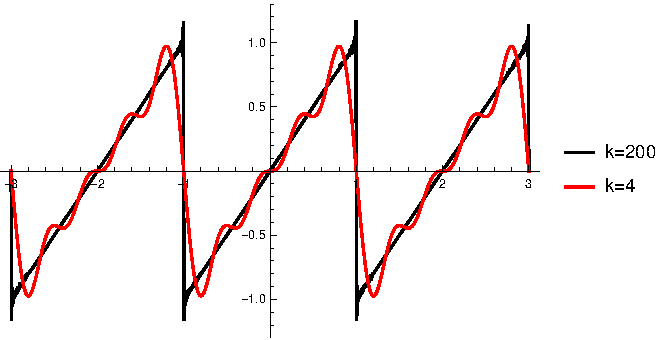
\includegraphics[width=\columnwidth]{images/sawtooth_series.pdf}\vfill
\raggedright Zoom in on discontinuity \vfill
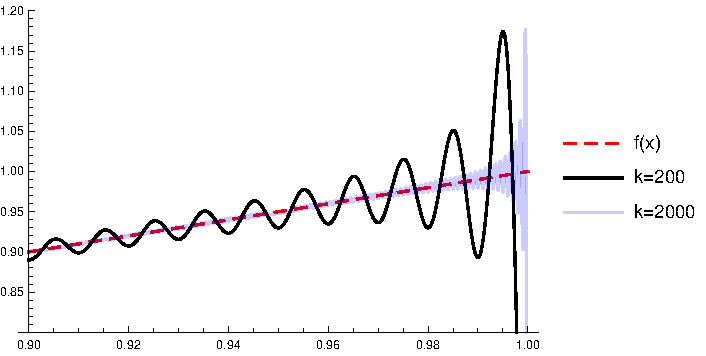
\includegraphics[width=\columnwidth]{images/sawtooth_zoom_in.pdf}
}{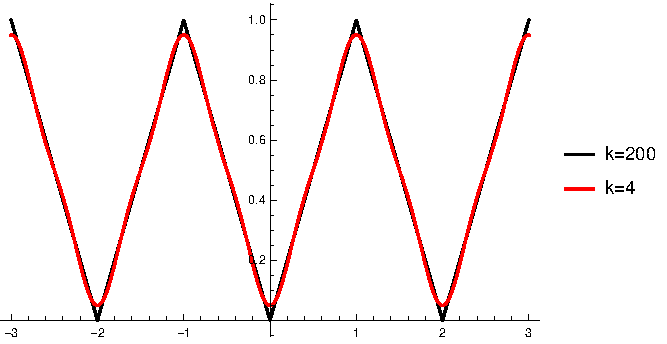
\includegraphics[width=\columnwidth]{images/triangle_series.pdf}\vfill
\raggedright Zoom in on discontinuity \vfill
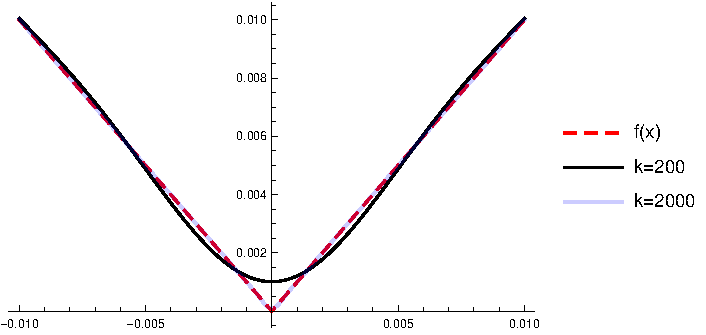
\includegraphics[width=\columnwidth]{images/triangle_zoom_in.pdf}}
}


\slide[Fourier Series Convergence]{

\itmz{\item The Fourier Series of any continuous function converges (as $k\to\infty$) to the function value at every point. $\Rightarrow f(x)=\text{FS}(f(x))$\vfill
\item The Fourier Series of a function with jump discontinuities exhibits \alert{Gibb's phenomena}\vfill
\subitem{High frequency over/undershooting of the function \\
\centerline{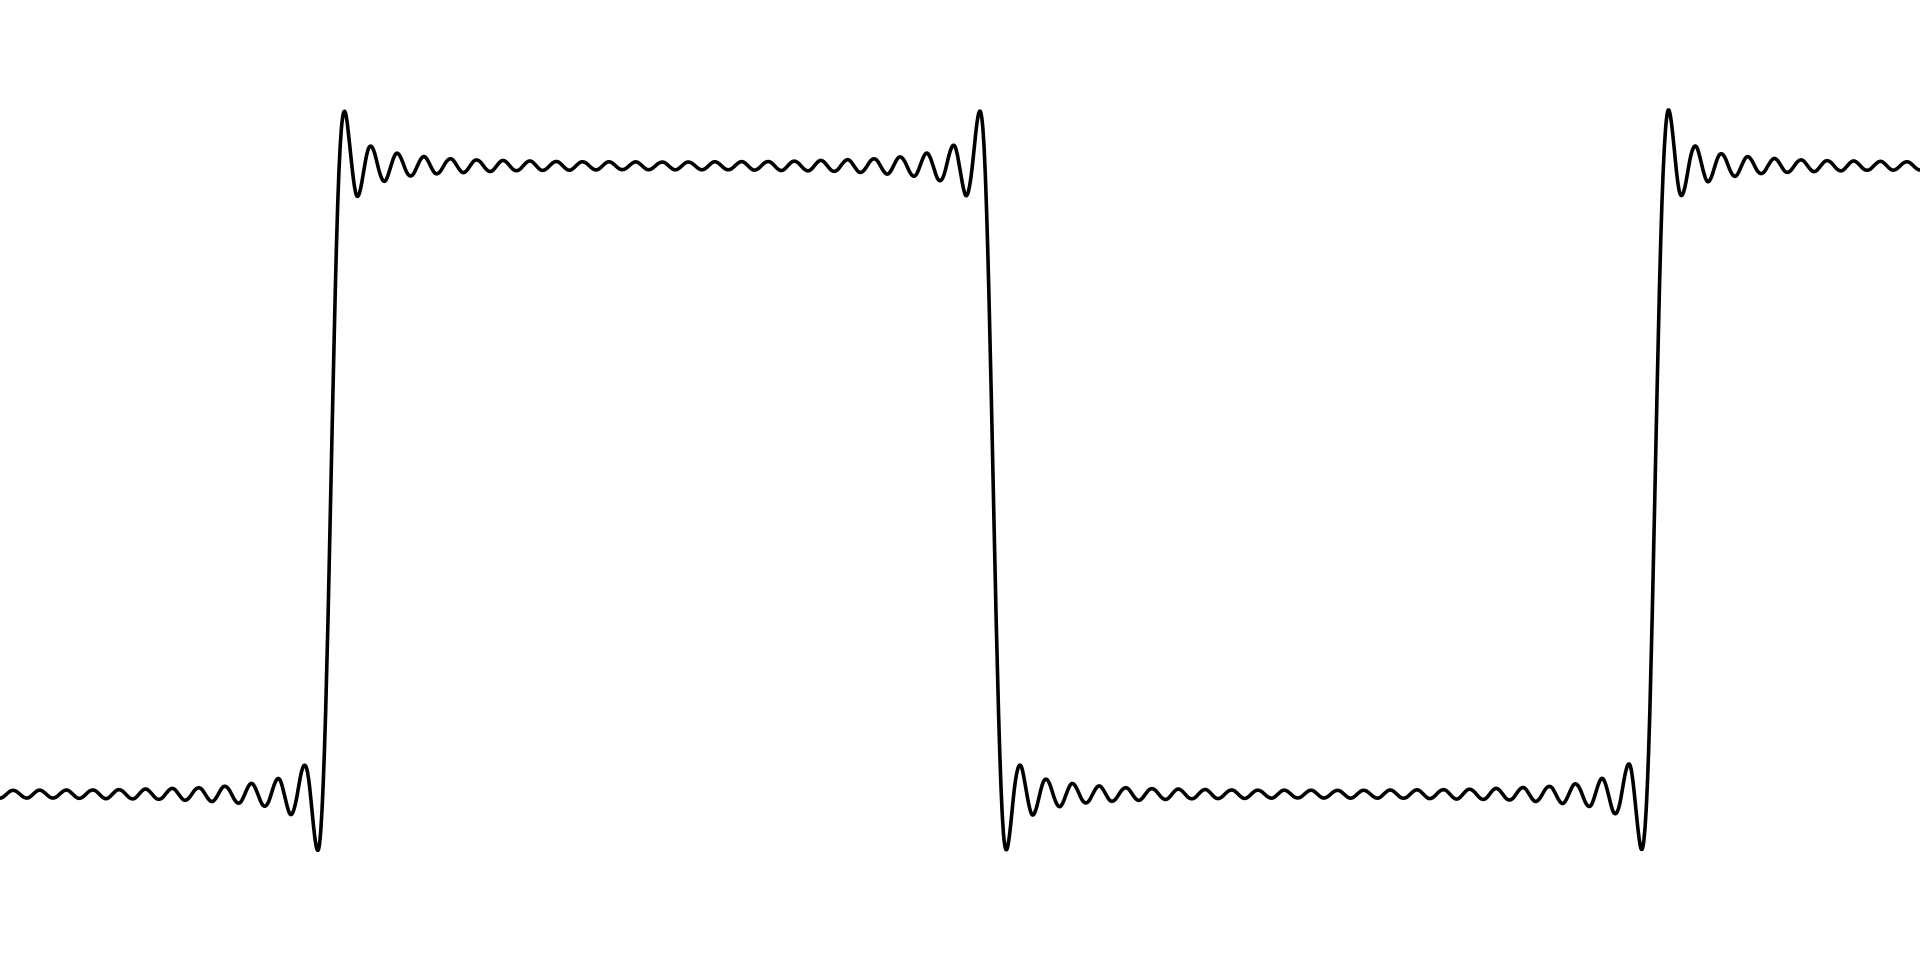
\includegraphics[width=4cm]{images/gibbs.png}}}\vfill
\item The Fourier Series converges to the midpoint between the two function values at any point of discontinuity. $\Rightarrow f(x)\approx \text{FS}(f(x))$\vfill
\item The rate of convergence of smooth functions is  faster than for functions with discontinuities.}

}

\end{document}